% xor.png -- the AND/XOR figure of sections 3.2 and 3.6.
% (a) AND: one line separates the single 1 from the three 0s.
% (b) XOR: every line puts at least one point on the wrong side. The best
%     line found by exhaustive search is the one drawn in (a) -- with its two
%     sides swapped -- so it keeps every point well away from the boundary and
%     loses exactly one of them, the bottom-left (0,0).
% (c) XOR with four sigmoid hidden neurons: the two solid curves are the
%     level set probability = 0.5 of the network trained in section 3.6.
% Build: bash tools/figures/build.sh
\documentclass[tikz,border=5pt]{standalone}
% Shared style for the neural-network diagrams in notebooks/img/nn-*.png.
% Palette and look are matched to the pre-existing figures (nn-1..nn-8,
% backprop-*) so a regenerated figure sits next to them unnoticed.
\usepackage[T1]{fontenc}
\usepackage{newtxtext}
\usepackage{newtxmath}
\usetikzlibrary{arrows.meta,calc,positioning}

\definecolor{innavy}{HTML}{004475}     % input neurons, source-like labels
\definecolor{hidyellow}{HTML}{FFCF6E}  % hidden neurons
\definecolor{outmaroon}{HTML}{8E1854}  % output neuron
\definecolor{accgold}{HTML}{E5A600}    % "Hidden Layer" label
\definecolor{gridgrey}{HTML}{B7B7B7}

\tikzset{
  neuron/.style   = {circle, draw=black, line width=0.9pt, minimum size=0.9cm,
                     inner sep=0pt, font=\large\bfseries},
  hidden/.style   = {neuron, fill=hidyellow},
  inputn/.style   = {neuron, fill=innavy, text=white},
  outputn/.style  = {neuron, fill=outmaroon, text=white},
  conn/.style     = {-{Latex[length=2.2mm,width=1.6mm]}, line width=0.7pt},
  bias/.style     = {-{Latex[length=1.8mm,width=1.3mm]}, line width=0.7pt},
  biaslbl/.style  = {font=\scriptsize, inner sep=1pt},
  layerlbl/.style = {font=\large\bfseries},
}

% Column positions shared by every figure (1 unit = 1cm).
\def\HIDX{3.4}   % hidden neurons
\def\ACTX{4.9}   % activation insets (centre)
\def\OUTX{7.4}   % output neuron
\def\NODE{0.45}  % neuron radius
\def\BOX{0.42}   % activation inset half-width

% Framed mini-plot of the sigmoid, drawn where the existing figures draw it.
% Usage: \actinset{x}{y}{label}
\newcommand{\actinset}[3]{%
  \begin{scope}[shift={(#1,#2)}]
    \fill[white] (-\BOX,-\BOX) rectangle (\BOX,\BOX);
    \foreach \g in {-0.14,0.14}{%
      \draw[gridgrey, line width=0.35pt] (-\BOX,\g) -- (\BOX,\g);
      \draw[gridgrey, line width=0.35pt] (\g,-\BOX) -- (\g,\BOX);}
    \draw[black, line width=1.1pt, domain=-0.40:0.40, samples=60]
      plot ({\x}, {0.78/(1+exp(-9*\x)) - 0.39});
    \draw[black, line width=0.9pt] (-\BOX,-\BOX) rectangle (\BOX,\BOX);
    \node[above left, font=\scriptsize, inner sep=1pt] at (\BOX,\BOX+0.02) {#3};
  \end{scope}}

% Bias arrow plus label above a neuron: \biasup{node name}
\newcommand{\biasup}[1]{%
  \draw[bias] ($(#1)+(0,\NODE+0.41)$) -- ($(#1)+(0,\NODE+0.01)$);
  \node[biaslbl, above] at ($(#1)+(0,\NODE+0.41)$) {Bias};}

% A vector collapsed into one node: two offset discs behind it.
% Usage: \vectornode{x}{y}{label}
\newcommand{\vectornode}[3]{%
  \foreach \dx/\dy in {0.13/0.11, 0.26/0.22}{%
    \draw[innavy, line width=0.7pt, fill=innavy!22]
      ($(#1,#2)+(\dx,\dy)$) circle (\NODE);}
  \node[inputn] (#3) at (#1,#2) {$#3$};}

\begin{document}
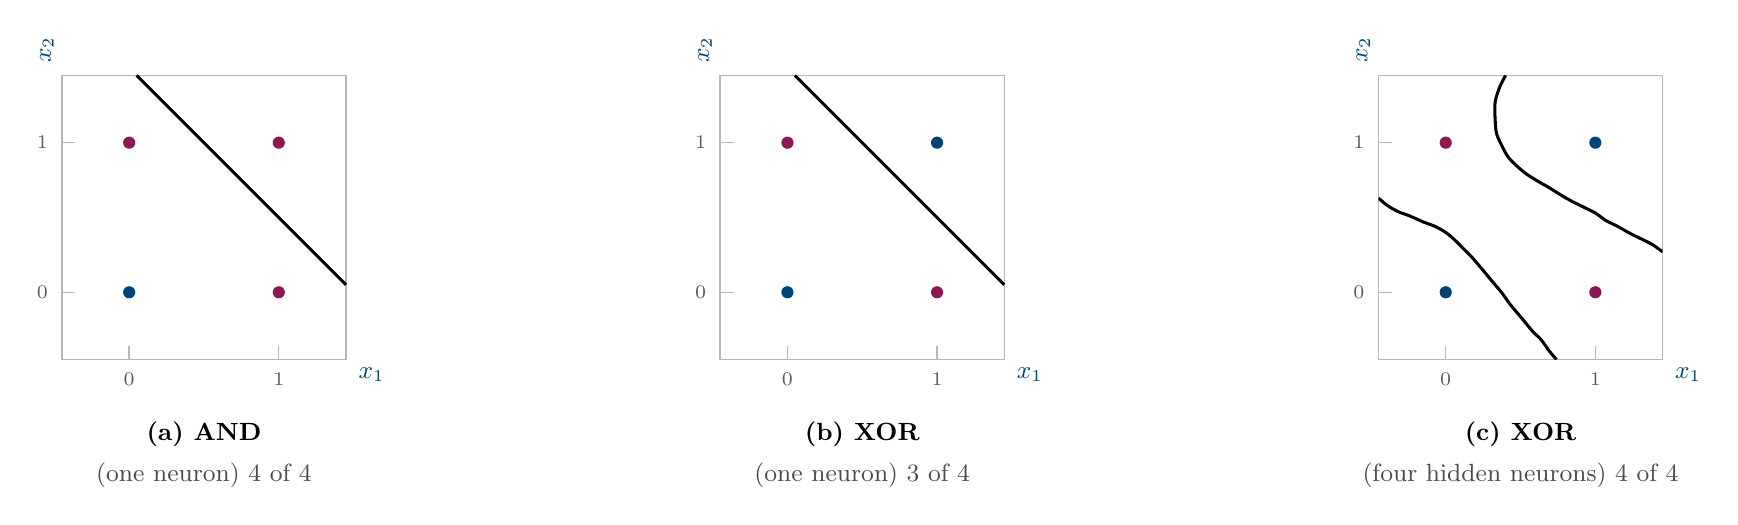
\begin{tikzpicture}[x=1.9cm,y=1.9cm]

% ---- shared drawing helpers -----------------------------------------------
% framed input square with 0/1 ticks
\newcommand{\gateframe}{%
  \draw[gridgrey, fill=white, line width=0.5pt] (-0.45,-0.45) rectangle (1.45,1.45);
  \foreach \v in {0,1}{%
    \draw[gridgrey, line width=0.5pt] (\v,-0.45) -- (\v,-0.36);
    \draw[gridgrey, line width=0.5pt] (-0.45,\v) -- (-0.36,\v);
    \node[font=\scriptsize, text=black!65] at (\v,-0.58) {\v};
    \node[font=\scriptsize, text=black!65] at (-0.58,\v) {\v};}}

% one training point: class 0 filled navy, class 1 filled maroon
\newcommand{\gpt}[2]{\fill[#1] (#2) circle (2.2pt);}

% panel title and score: \gcapt{shift}{title}{score}
\newcommand{\gcapt}[3]{%
  \node[font=\small\bfseries, align=center] at ($(#1)+(0.5,-0.95)$) {#2};
  \node[font=\small, text=black!70] at ($(#1)+(0.5,-1.22)$) {#3};}

% =========================== (a) AND =======================================
\begin{scope}[shift={(0,0)}]
  \gateframe
  \draw[black, line width=1.1pt] (1.45,0.05) -- (0.05,1.45);
  \gpt{innavy}{0,0}
  \gpt{outmaroon}{0,1}
  \gpt{outmaroon}{1,0}
  \gpt{outmaroon}{1,1}
\end{scope}
\gcapt{0,0}{(a) AND}{(one neuron) 4 of 4}

% =========================== (b) XOR, one neuron ===========================
\begin{scope}[shift={(4.4,0)}]
  \gateframe
  \draw[black, line width=1.1pt] (1.45,0.05) -- (0.05,1.45);
  \gpt{innavy}{0,0}
  \gpt{outmaroon}{0,1}
  \gpt{outmaroon}{1,0}
  \gpt{innavy}{1,1}
\end{scope}
\gcapt{4.4,0}{(b) XOR}{(one neuron) 3 of 4}

% =========================== (c) XOR, hidden layer =========================
\begin{scope}[shift={(8.8,0)}]
  \gateframe
  \begin{scope}
    \clip (-0.45,-0.45) rectangle (1.45,1.45);
    % probability = 0.5, upper branch
    \draw[black, line width=1.1pt]
      plot[smooth] coordinates {
        (1.45,0.27) (1.38,0.32) (1.30,0.36) (1.22,0.40) (1.15,0.44)
        (1.07,0.48) (1.00,0.53) (0.92,0.57) (0.84,0.61) (0.77,0.65)
        (0.69,0.70) (0.62,0.74) (0.54,0.79) (0.48,0.84) (0.42,0.90)
        (0.38,0.97) (0.34,1.06) (0.33,1.16) (0.33,1.27) (0.36,1.37)
        (0.40,1.45)};
    % probability = 0.5, lower branch
    \draw[black, line width=1.1pt]
      plot[smooth] coordinates {
        (-0.45,0.63) (-0.39,0.58) (-0.32,0.54) (-0.24,0.51) (-0.15,0.47)
        (-0.07,0.44) (-0.00,0.40) (0.06,0.35) (0.12,0.29) (0.17,0.24)
        (0.23,0.17) (0.28,0.11) (0.33,0.05) (0.38,-0.01) (0.43,-0.08)
        (0.48,-0.14) (0.53,-0.20) (0.58,-0.26) (0.64,-0.32) (0.69,-0.39)
        (0.74,-0.45)};
  \end{scope}
  \gpt{innavy}{0,0}
  \gpt{outmaroon}{0,1}
  \gpt{outmaroon}{1,0}
  \gpt{innavy}{1,1}
\end{scope}
\gcapt{8.8,0}{(c) XOR}{(four hidden neurons) 4 of 4}

% axis names, placed outside the frame so they never cross the data
\foreach \dx in {0,4.4,8.8}{%
  \node[font=\small, text=innavy] at ($(\dx,0)+(1.62,-0.55)$) {$x_1$};
  \node[font=\small, text=innavy, rotate=90] at ($(\dx,0)+(-0.55,1.62)$) {$x_2$};}

\end{tikzpicture}
\end{document}
